\section{Super-Resolution}

\noindent Ein \ac{GAN}, welches trainiert wurde, um das Prinzip der Super-Resolution anzuwenden, generiert statt neuen Bildinhalten eine verbesserte Version des Originals mit erweiterter visueller Qualität. Diese Verbesserung kann in unterschiedlichen Formen auftreten, beispielsweise durch eine höhere Auflösung, eine verbesserte Farbgebung, Entfernen von Rauschen und Schmutz, sowie das Schärfen der Bilder. Im unteren Beispiel \ref{fig:scaling} ist eine Demonstration einer Super-Resolution-GAN zu sehen, welche ein herunterskaliertes Bild auf die ursprüngliche Auflösung hochskaliert. Dabei ist zu beobachten, dass die KI die hochfrequenten Details wie die zerfransten Kanten nicht replizieren kann und das Resultat sehr geglättet wird. Dies liegt daran, dass diese Information durch das Herunterskalieren irreparabel verloren gegangen ist und die KI lediglich raten kann, wie das Bild ursprünglich aussah.\\


\begin{figure}[H]
    \centering
    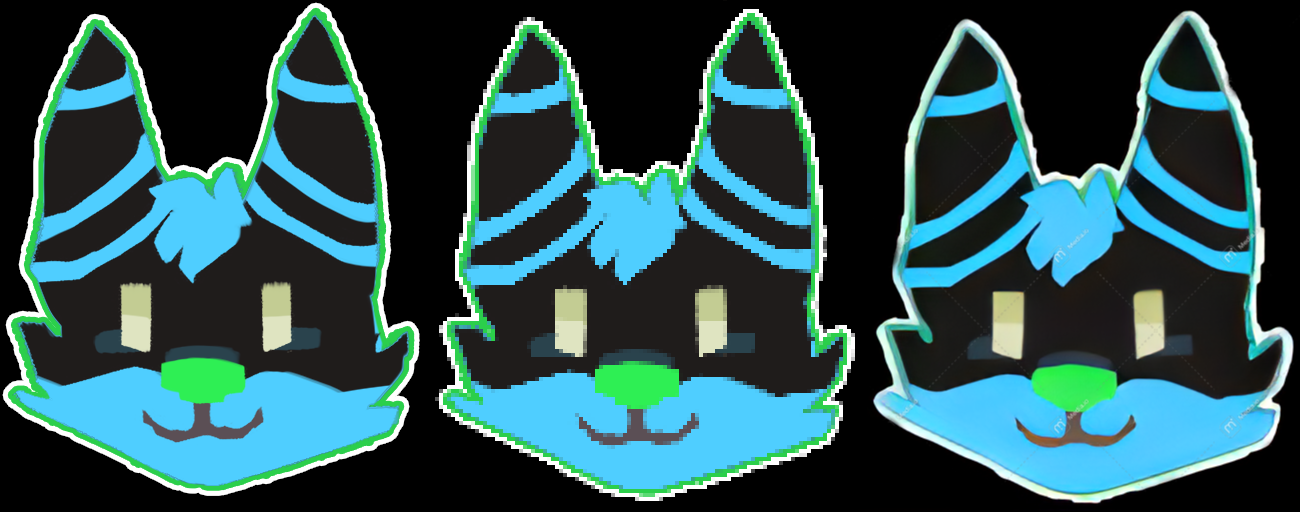
\includegraphics[width=1\textwidth]{scaling}
    \caption{Demonstration Super-Resolution-GAN: Originalbild (links), verkleinertes Original (Mitte) und per KI restaurierte Version (rechts, mit Wasserzeichen)} \quelle\url{https://imgupscaler.media.io}
\label{fig:scaling}
\end{figure}


\noindent Auch bei Videos kann das Prinzip angewendet werden, wobei eine Verbesserung intra-frame stattfinden kann, das heißt die einzelnen Standbilder können visuell optimiert werden, doch Bewegtbilder bieten ebenfalls die Möglichkeit, Optimierungen inter-Frame durchzuführen. Genauer gesagt bedeutet dies, dass die oben genannten Verbesserungen wie höhere Auflösung und Optimierung des Bildinhalts nicht nur auf den zweidimensionalen Raum, sondern ebenfalls auf den dreidimensionalen Raum angewendet werden kann, wobei die dritte Achse die Zeit darstellt. So kann beispielsweise die Bildwiederholungsrate erhöht werden, indem zwischen Bildern interpoliert wird, was die Bewegungen weicher und flüssiger aussehen lässt.
\newpage